% !TeX encoding = UTF-8
% !TeX spellcheck = sk_SK
% !TeX root=teoriaprocesovtakac.tex
\section{Kyslíkový konvertor}

V oceliarstve nastal počas druhej polovice 20. storočia významný posun a progres vo~vývoji technológií a procesov výroby ocele. Jedným z najdôležitejších milníkov bolo prvé spustenie komerčnej prevádzky výroby ocele vháňaním kyslíka do konvertora začiatkom 50. rokov minulého storočia v mestách Linz (firma VÖEST) a~Donawitz (forma ÖAMG) v Rakúsku. Z názvov týchto miest pochádza aj pomenovanie spôsobu výroby ocele praktizovanom v kyslíkových konvertoroch, a to LD proces, a~zároveň aj názov samotného kyslíkového konvertora (LD konvertor). LD proces je vo svete široko preferovaná a efektívna metóda výroby ocele vďaka vysokej produktivite a~značne nízkym výrobným nákladom \cite{Wang2010}.

Postupom času a zdokonaľovaním tohto procesu sa LD konvertory rozšírili do~celého sveta a už niekoľko rokov sú najvyužívanejšou technológiou pre výrobu ocele na celom svete (až 65\% podiel tejto metódy pre tavbu surovej ocele).

\begin{figure}[h!]
\centering
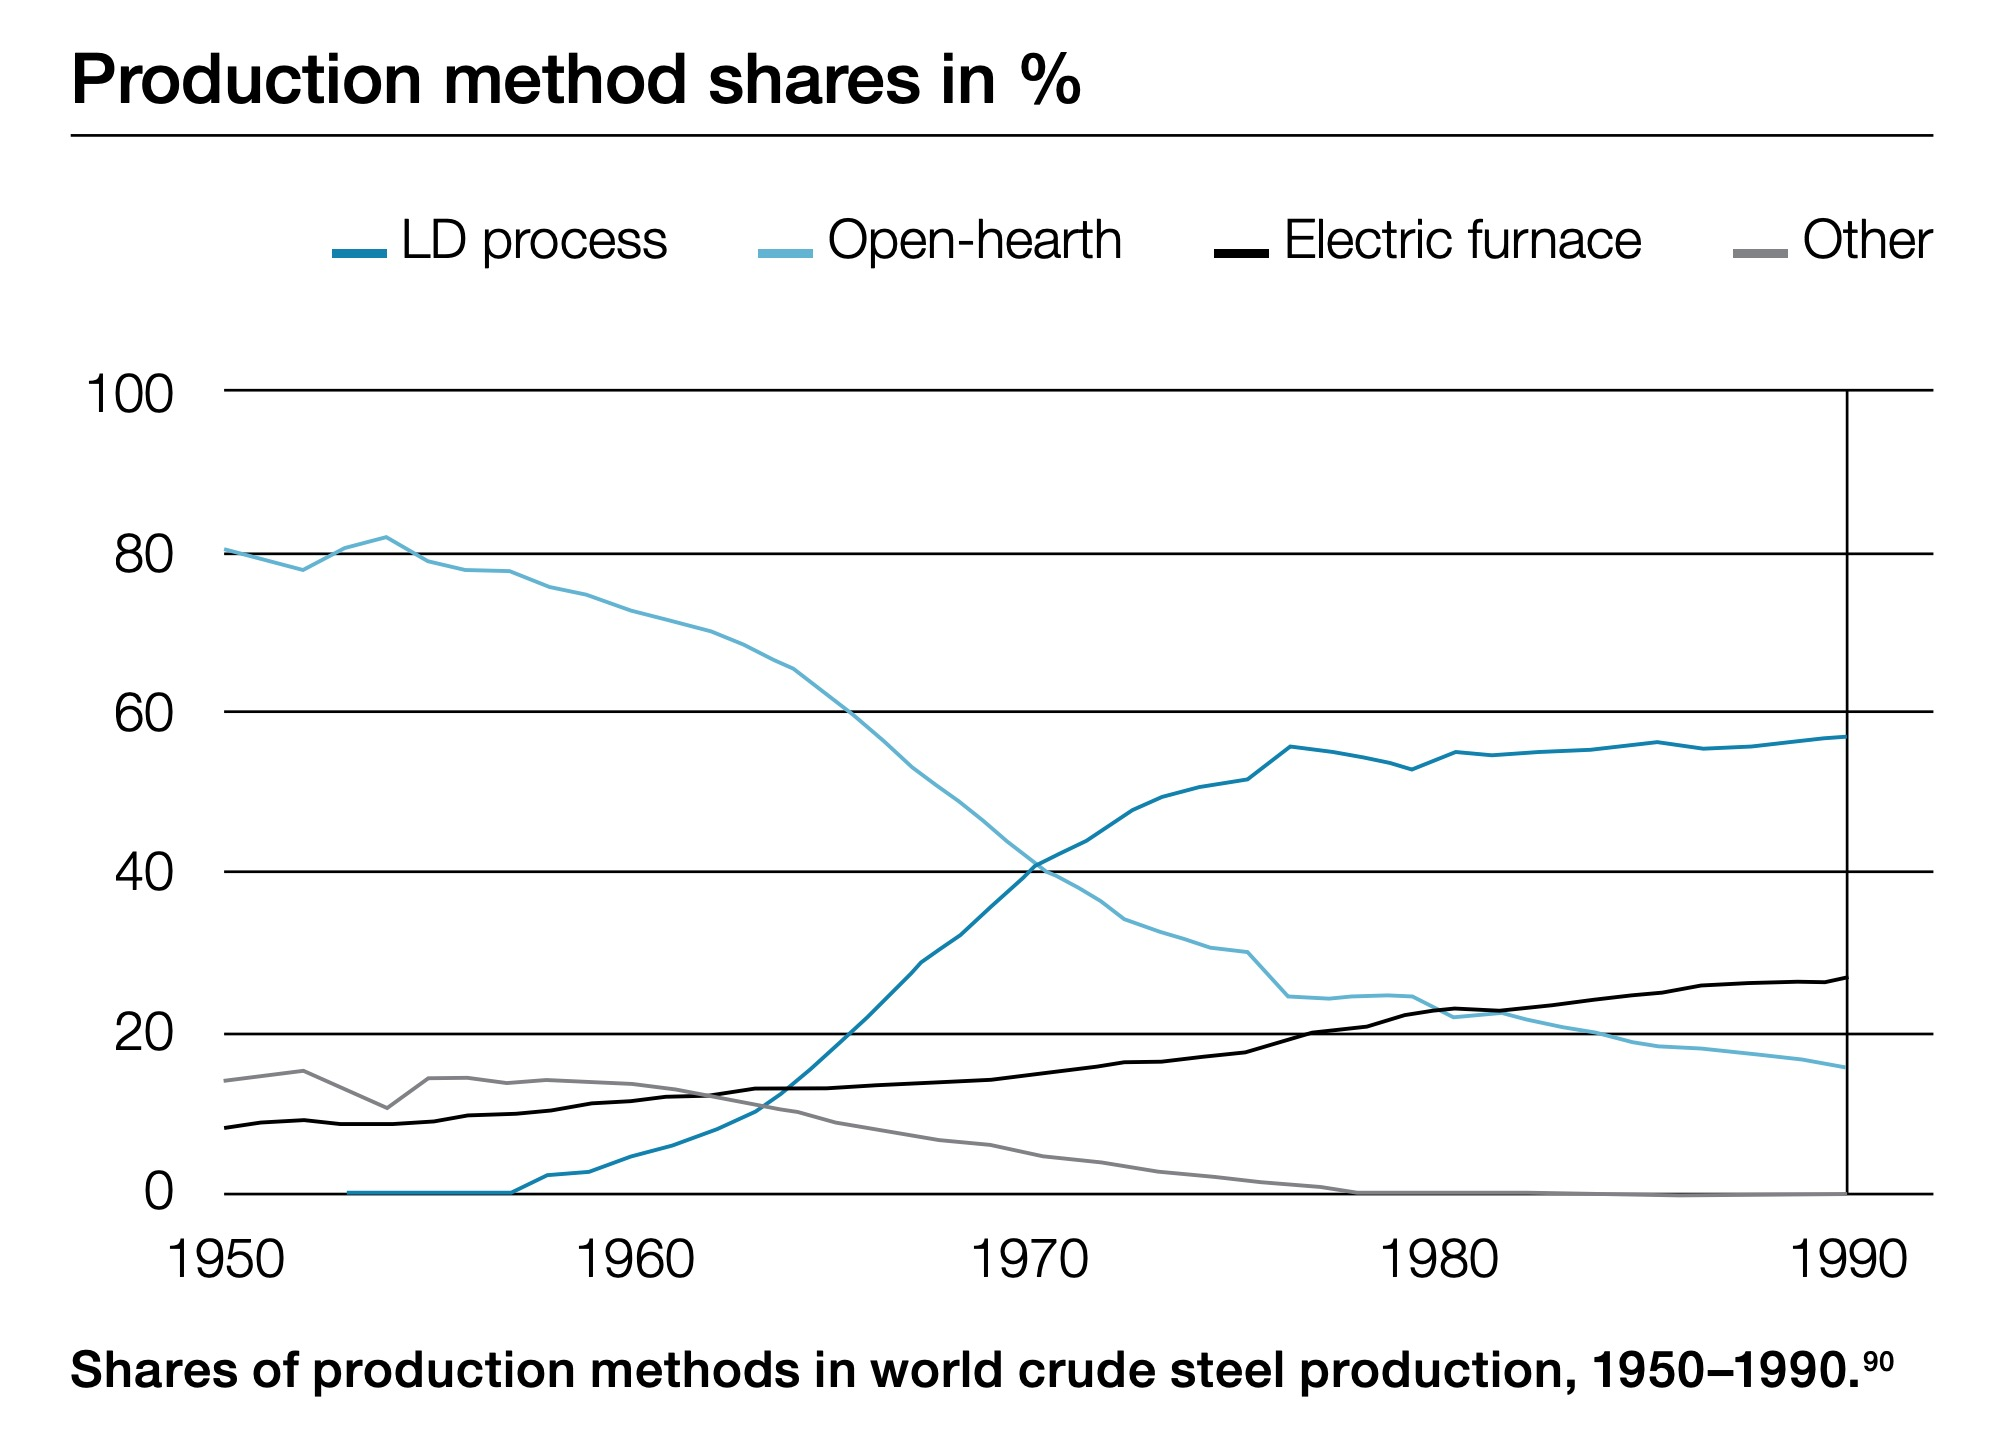
\includegraphics[width=.9\textwidth,angle=0]{ld-process-history-data.jpg}
\caption{Podiel výrobných metód ocele v percentách \citep{voestalpineLD2012}}
\label{o:1}
\end{figure}

Spomínaný LD proces sa v rôznych častiach sveta nazýva odlišne. Napríklad vo~Veľkej Británii sa označuje ako BOS (basic oxygen steelmaking); v~Amerike a~v~Ázijských krajinách BOF (basix oxygen furnace) s výnimkou americkej korporácie U.S. Steel, kde sa často označuje ako BOP (basic oxygen process) \citep{Turkdogan1996}.

\begin{figure}[h!]
\centering
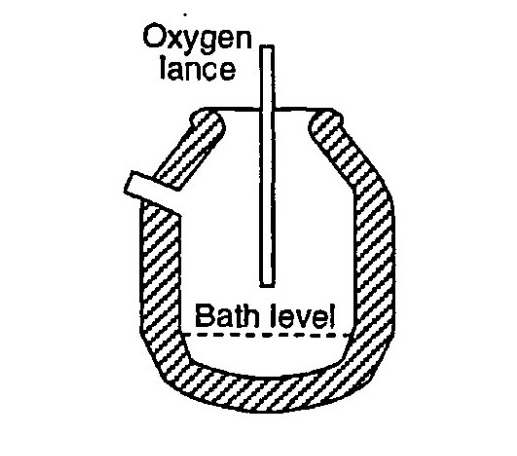
\includegraphics[width=.4\textwidth,angle=0]{bof-single.jpg}
\caption{Výroba ocele v konvertore fúkaním kyslíka zhora (LD/BOF) \citep{Turkdogan1996}.}
\label{o:2}
\end{figure}

V 70. rokoch bol v Kanade a Nemecku vyvinutý upravený typ konvertora s~vháňaním kyslíka z dolnej časti, ktorý bol následne komercializovaný. Tento proces sa v Európe označuje ako OBM a v iných častiach sveta ako Q-BOP.

\begin{figure}[h!]
\centering
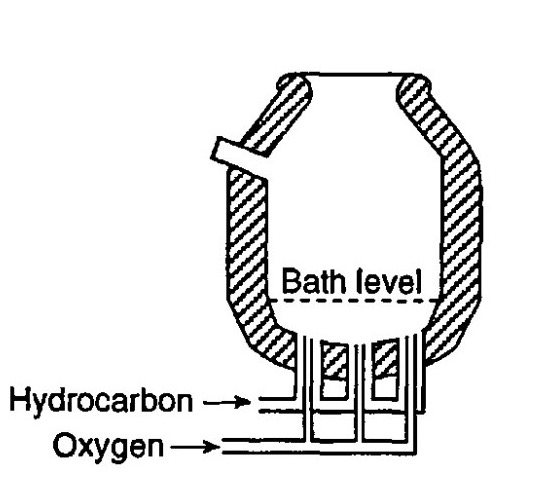
\includegraphics[width=.4\textwidth,angle=0]{q-bop.jpg}
\caption{Výroba ocele v konvertore fúkaním kyslíka zdola (Q-BOP) \citep{Turkdogan1996}.}
\label{o:3}
\end{figure}

V konvertore pre Q-BOP proces sa v dolnej časti nachádzajú trysky vsadené do odnímateľného dna, cez ktoré je vháňaný kyslík (\ce{O2}) spolu s páleným vápnom cez prstencovú medzeru okolo centrálnej rúry sa privádza plynný uhľovodík (napr. propán alebo metán). Po kontakte s tekutou oceľou uhľovodík disociuje na \ce{C} a \ce{H2} pri absorpcii tepla. Táto endotermická reakcia potláča prehrievanie hrotu trysky exotermickou reakciou kyslíka s~tekutou oceľou.

Ďalší vývojovým krokom výroby ocele v~kyslíkovom konvertore bolo spojenie typov fúkania kyslíka zhora a~zdola.

\begin{figure}[h!tbp]
\centering
\subfloat[Kombinovaný BOF.]{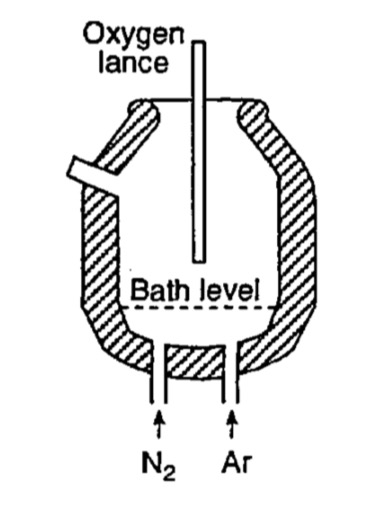
\includegraphics[width=0.38\textwidth]{kombinovany-bof.jpg}\label{fig:f1}}
\hfill
\subfloat[Kombinovaný Q-BOP.]{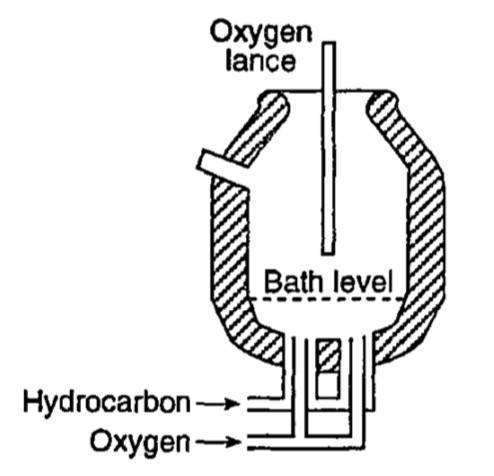
\includegraphics[width=0.52\textwidth]{kombinovany-q-bop.jpg}\label{fig:f2}}
\caption{Výroba ocele procesom BOF a Q-BOP v LD konvertore s kombinovaným typom fúkania.}
\label{o:4}
\end{figure}

